\documentclass[a4paper, 12pt]{report}

\usepackage[utf8]{inputenc}
\usepackage[T1]{fontenc}
\usepackage[francais]{babel}
\usepackage{graphicx}
\usepackage{amsmath}
\usepackage{amsfonts}
\usepackage{amssymb}

\title{LO41 - Gestion des voies ferroviaires}
\author{Staine Florian}
\date\today

\begin{document}
\maketitle

\chapter{Objectif}
L'objectif de ce projet est de mettre en pratique les aspects de synchronisation, communication, multiprogrammation ou encore inter-blocage qui peuvent intervenir 
lors de la réalisation de certains programmes informatiques.

\section{Problème à résoudre}
Pour mettre en pratique les différentes thématiques citées plus haut, 
l'objectif est de concevoir un système permettant de gérer le déplacement de trains 
sur différentes voies ferroviaires.\\
Les voies diffèrent selon le type de train qui peut circuler dessus, le nombre maximum de train admissibles par voie ainsi que le sens de circulation.\\
Les voies se connectent ensuite entres elles pour permettre à tous les trains d'atteindre l'autre coté de l'aiguillage. \\
Une certaine priorité est mise en place entre les différents trains :

\begin{enumerate}
\item TGV
\item Grandes Lignes
\item Marchandises\newline{}
\end{enumerate}

Les TGV présents seront prioritaires sur les autres, dans la mesure du possible.
C'est à dire que l'on tentera de libérer les trains les plus prioritaires en premiers, 
mais si un train est engagé sur une voie, il ne faut pas en libérer un autre 
dans le sens inverse, même si celui-ci serait plus prioritaire, 
sous peine de créer un inter-blocage.
Cela conduirait le système tout entier à être bloqué sans issue possible.

\section{Modélisation}

\subsection{Modélisation du tunnel}
\begin{figure}[hbtp]
\centering
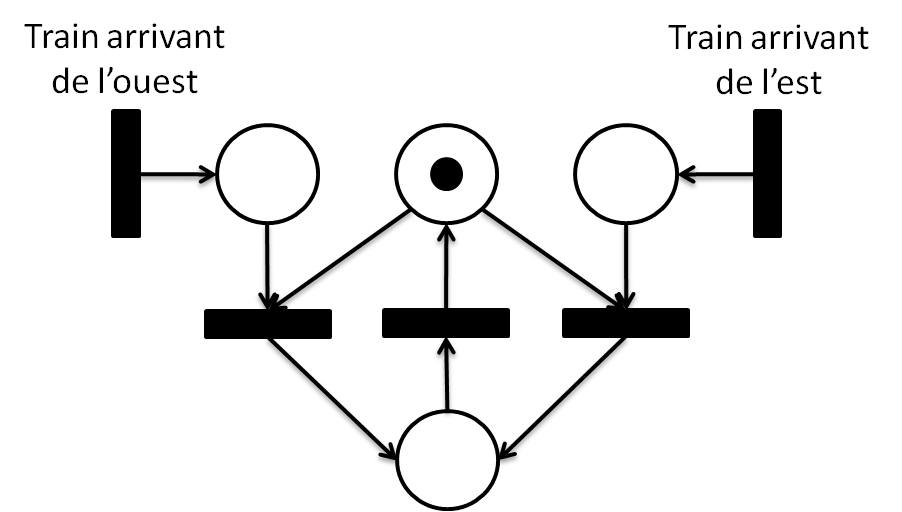
\includegraphics[width=8cm]{Tunnel.png}
\caption{Réseau de pétri du tunnel}
\end{figure}

Les réseaux représentant les autres segements de voieries n'étant pas fonctionnels, ils n'ont pas été ajoutés au rapport. 

\chapter{Implémentation}
\section{Structure générale}
Le programme s'appuie sur l'utilisation de threads pour représenter les différentes entités. \\
Un premier thread aiguilleur est créer et initialise la voie. Il est ensuite en permanence à la recherche de trains à libérer.\\ \newline{}
Chaque train est représenté par un thread autonome qui se réfère au thread aiguilleur pour recevoir les autorisations d'accès. 
Tant qu'il ne peut pas s'arrêter sur sa voie actuelle, il continue son avancée 
en vérifiant s'il ne rentre pas en collision avec un autre train.\\
Enfin, un dernier thread s'occupe de l'affichage de l'aiguillage. 
L'affichage est remis à jour à chaque période, une période correspondant au temps nécessaire à un train pour passer d'une voie à une autre. \\ \newline{}
Il n'y a pas de surcharge des actions des signaux car le programme ne contient rien qui doit être libéré 
(car pas d'utilisation de malloc, ni d'objets IPC qui seraient persistants.)

\section{Initialisation}
Au démarrage du programme, l'aiguillage est créé, les voies et leurs mutex sont initialisées.
Ensuite, tous les trains sont générés et lancés par des threads différents.
Les 10 premiers trains sont définis manuellement (pour permettre de faire des tests) et les autres sont initialisés avec un sens et un type aléatoires.
La position du train est ensuite attribuée en fonction du sens du train, puis celui-ci est lancé sur l'aiguillage.

\section{Gestion des sections critiques et synchronisation}
Les sections critiques et ressources partagées sont protégées par l'utilisation de moniteurs. 
Chaque voie possède son propre mutex ainsi que trois conditions, 
permettant de libérer les différents types de trains. 
Il y a également un mutex permettant de signaler que l'aiguillage est prêt à être utilisé 
et donc que les trains peuvent commencer à être générés, 
ainsi qu'un mutex permettant à l'affichage de l'aiguillage de ne pas être coupé 
par un autre affichage qui se ferait en même temps. 

\section{Libération des trains}
Un aiguilleur gère toutes les voies en libérant des trains possibles, 
le tout en évitant, bien évidement, inter-blocages et collisions. \\

Toutes les voies ne permettent pas un arrêt des trains dessus. 
Les trains ne se mettent donc pas toujours en attente avant de passer sur la voie suivante, 
mais continuent leur chemin tout en contrôlant qu'il n'y aie pas d'inter blocage avec un train arrivant en face.\\
Sur les voies autorisant les arrêts, les trains sont automatiquement bloqués à leur arrivée, puis ils attendent d'être libérés par l'aiguilleur.
Pour cela, ils se mettent en attente sur la condition de la voie correspondant à leur type 

\chapter*{Conclusion}
\section{Limites du programme}
\subsection{Réseau non modulaire}
En cas de modification du réseau ferroviaire, 
il faudrait apporter d'importantes modifications au programme gérant l'aiguillage pour que les trains soient libérés correctement. 
En effet, les fonctions qui permettent la libération d'une voie ne sont pas génériques, 
ce qui signifie que s'il on rajouter une voie il faut modifier plusieurs fonctions de libération pour prendre en compte le changement. 

\section{Problèmes rencontrés}
\subsection{Modélisation par réseaux de Pétri}
Lors de la partie modélisation, les réseaux de Pétri réalisés ne correspondaient pas au modèle voulu.\\
N'aidant pas à comprendre la problématique, ils n'ont pas été ajoutés au rapport. 

\section{Améliorations possibles}
\subsection{Unification des fonction de libération}
Il serait beaucoup plus simple et élégant de gérer un modèle générique de voie et 
de libération permettant de prendre en compte les éléments de voieries sans avoir à définir manuellement le comportement de l'aiguilleur. 
Il serait alors beaucoup plus aisé de retirer, d'ajouter, ou encore de modifier les paramètres de voies. 

\subsection{Séparation des trains et de l'aguilleur}
Dns ce projet, les trains sont gérés à l'intérieur de l'aiguilleur, ce qui est plus simple car ainsi 
l'aiguilleur peut à tout moment connaitre l'état des trains.
Dans la réalité, les trains sont autonomes et se réfèrent à l'aiguilleur 
en lui envoyant les informations nécessaires au bon fonctionnement de l'ensemble.

\end{document}
